\documentclass[11pt]{beamer}
\usetheme{Madrid}
\usepackage[utf8]{inputenc}

\usepackage[english]{babel}

\usepackage{amsmath}
\usepackage{amsfonts}
\usepackage{amssymb}
\usepackage{graphicx}

\usepackage{graphicx}
\graphicspath{ {figures/} }
\usepackage{array}




\institute[]{Department of Banking \& Finance \\ Digital Tools for Finance \\ Dr. Igor Pozdeev \\} 

\author[Huser, Neller and Tassone]{Naomi Huser, 17-056-201 \\
Jonas Neller, 21-730-676 \\ Lorena Tassone, 18-700-237 }

\title[]{The Effect of U.S. Real
        GDP on different S\&P500 sector indices' market capitalizations}




\setbeamertemplate{navigation symbols}{}
\setbeamertemplate{caption}[numbered]
\institute[]{University of Zurich \\ Department of Banking \& Finance \\ Digital Tools for Finance \\ Dr. Igor Pozdeev \\} 
\date{December 19, 2022} 


\bibliographystyle{apalike}



\begin{document}

\begin{frame}
\titlepage
\end{frame}

\begin{frame}{Summary}
\tableofcontents 
\end{frame}

\section{Introduction}
\begin{frame}{Introduction}
   Multiple macroeconomic factors suspected to influence stock market activities:

    \begin{itemize}
        \item Real GDP
        \item Unemployment Rate
        \item Crude Prices
        \item Federal Debt 
        \item Federal Rate
    \end{itemize}
    
    \bigskip
    
    Factors, which affect the financial markets most likely to have influence on market capitalization values.

\end{frame}

\section{Research Question}

\begin{frame}{Research Question}

"What is the effect of U.S. Real GDP on different S\&P500 sector indices' market capitalization?"
   
\end{frame}

\section{Data}

\begin{frame}{Data}

Quarterly Paneldata, 2007 - 2021
\begin{itemize}
        \item Market Capitalization of all the companies listed in the S\&P500 Index in Million U.S. Dollars (Bloomberg\footnote{As an approximation of the index, we used the constituents of the iShares Core S\&P 500 UCITS ETF})
        \item All Macroeconomic Factors either expressed in percentage points or Million U.S. Dollars (FRED)
    \end{itemize}

\end{frame}

\section{Regression Model}
\begin{frame}{Regression Model}
For each sector:
\begin{equation}
  Y_t^{sector} = \beta_0 + \beta_1 X_{1,t} + \beta_2 X_{2,t} + \beta_3 X_{3,t} + \beta_4 X_{4,t} + \beta_5 X_{5,t} + u_t 
\end{equation}
   
\end{frame}

\begin{frame}{Regression Model}
\begin{table}
\caption{Variable Description}
\label{}
\begin{center}
\small

\begin{tabular}{ c c } \hline\hline
\hd{Variable in Model} & \hd{Representative for} \\ \hline\hline
$Y_t^{sector}$ & Average Sector Market Capitalization \\ \hline
$X_{1,t}$ & U.S. Real GDP (mio.) \\ \hline
$X_{2,t}$ &U.S. Unemployment Rate \\ \hline
$X_{3,t}$ &U.S. Crude Prices (mio.)  \\ \hline
$X_{4,t}$ &U.S. Federal Debt (mio.)  \\ \hline
$X_{5,t}$ &U.S. Federal Rate  \\ \hline
$\beta_0$ &Constant  \\ \hline
$\beta_1$ &Coefficient of U.S. Real GDP  \\ \hline
$\beta_2$ &Coefficient of U.S. Unemployment Rate  \\ \hline
$\beta_3$ &Coefficient of U.S. Crude Prices  \\ \hline
$\beta_4$ &Coefficient of U.S. Federal Debt \\ \hline
$\beta_5$ &Coefficient of U.S. Federal Rate \\ \hline
$u_t$  &Error Term \\ \hline
\hline
\end{tabular}
\end{center}
\end{table}
\end{frame}

\section{Regression Outputs}
\begin{frame}{Regression Outputs}

\begin{table}
\caption{Regression Outputs (1/2)}
\label{table:1}
\begin{center}
\tiny
\begin{tabular}{lllllll} \hline                  & Communication & Consumer Discretionary & Consumer Staples & Energy  & Financials  \\  \hline 
Intercept          & -426623.13***     & -101575.7*      & 63161.8*        & 140636.60*  & -61152.26    \\                    & (131825.81)       & (53595.73)       & (33392.26)       & (75401.66)  & (49080.77)     \\  
Real GDP          & 0.026***           & 0.005             & -0.003            & -0.005       & 0.005          \\                   & (0.009)            & (0.004)           & (0.002)           & (0.005)      & (0.004)           \\  
Unemployment rate & 1384.53           & 345.46           & -1996.10***      & -4172.22*** & -1083.3        \\                    & (1875.38)         & (762.46)         & (475.04)         & (1072.68)   & (698.23)        \\  
Crude price       & -225.78***        & 10.86           & -26.06           & 293.33***   & 4.13   \\                    & (69.59)           & (28.29)          & (17.63)          & (39.80)     & (25.91)    \\ 
Federal debt      & 0.004*             & 0.003***          & 0.003***          & 0.0009        & 0.001        \\                   & (0.002)            & (0.0009)           & (0.0006)           & (0.001)      & (0.0008)        \\ 
Federal rate      & 6599.31***        & 3160.23***       & 959.4**         & -923.95     & 2118.24***    \\                    & (1593.94)         & (648.04)         & (403.76)         & (911.70)    & (593.5)     \\ \hline  
R-squared          & 0.9673              & 0.9473             & 0.9611             & 0.73        & 0.93         \\  
R-squared Adj.     & 0.96              & 0.94             & 0.96             & 0.7        & 0.92         \\ \hline
\end{tabular}
\end{center}
\end{table}
\end{frame}

\begin{frame}{Regression Outputs}

\begin{table}
\caption{Regression Outputs (2/2)}
\label{}
\begin{center}
\tiny
\begin{tabular}{llllllll}  \hline                    &  Health Care & Industrials & Information Tech. & Materials & Real Estate & Utilities  \\  \hline 
Intercept             & -40738.04      & 13095.09        & -100640.41          & -12439.71     & -29193.64**    & -24398.88      \\                      & (35376.81)     & (23911.53)      & (139211.18)         & (14591.8)    & (12536.17)     & (16485.33)     \\  
Real GDP            & 0.0025           & -0.0006           & 0.0008                & 0.0007          & 0.002**         & 0.002           \\                     & (0.003)         & (0.002)          & (0.01)              & (0.001)        & (0.0009)         & (0.001)         \\  
Unemployment rate     & -590.88        & -1244.28***     & 2037.27             & -160.34       & -370.10**      & -61.43         \\                        & (503.28)       & (340.17)        & (1980.44)           & (207.59)      & (178.34)       & (234.52)       \\  
Crude price              & -51.38***      & 34.42***        & 58.77             & 38.74***      & -8.08          & -7.1          \\                       & (18.67)        & (12.62)         & (73.49)             & (7.70)        & (6.62)         & (8.70)         \\  
Federal debt            & 0.002***        & 0.002***         & 0.01***             & 0.0007***       & 0.0009***        & 0.0008***        \\                        & (0.0006)         & (0.0004)          & (0.002)              & (0.0002)        & (0.0002)         & (0.0003)         \\  
Federal rate        & 2100.13***     & 1395.31***      & 8851.46***          & 572.21***     & 375.95**       & 1085.08***     \\                  & (427.75)       & (289.12)        & (1683.24)           & (176.43)      & (151.58)       & (199.33)       \\ \hline  
R-squared           & 0.97           & 0.95            & 0.89                & 0.93          & 0.98           & 0.96           \\   
R-squared Adj.              & 0.97           & 0.94            & 0.88                & 0.92          & 0.98           & 0.95          \\  \hline  \\
\end{tabular}
\end{center}
\end{table}
\end{frame}

\section{Graphs}
\begin{frame}{Graphs}

Communication Services:
  \begin{figure}
    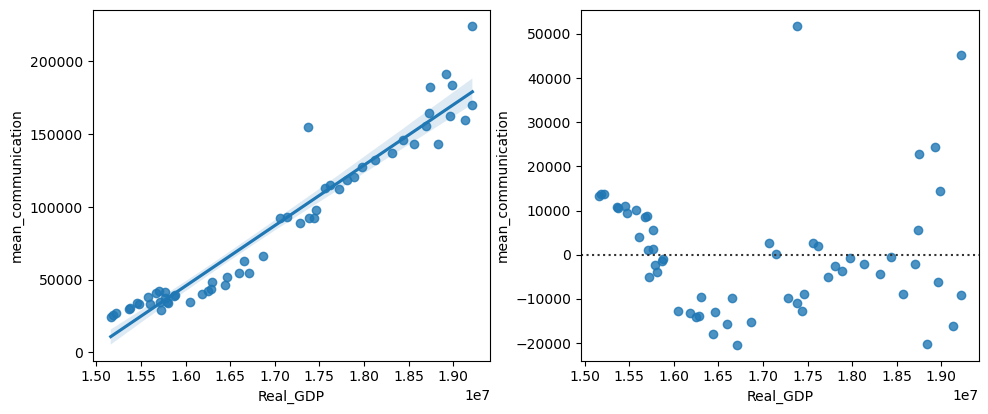
\includegraphics[width=1\textwidth]{imagens/Communication_Services.png}
    \caption{Regression and residual plot for the Communication Services sector}
    \label{something}
  \end{figure}
  
\begin{itemize}
    \item Positive significant effect
    \item No homoscedasticity
\end{itemize}
\end{frame}


\begin{frame}{Graphs}
Real Estate:
  \begin{figure}
    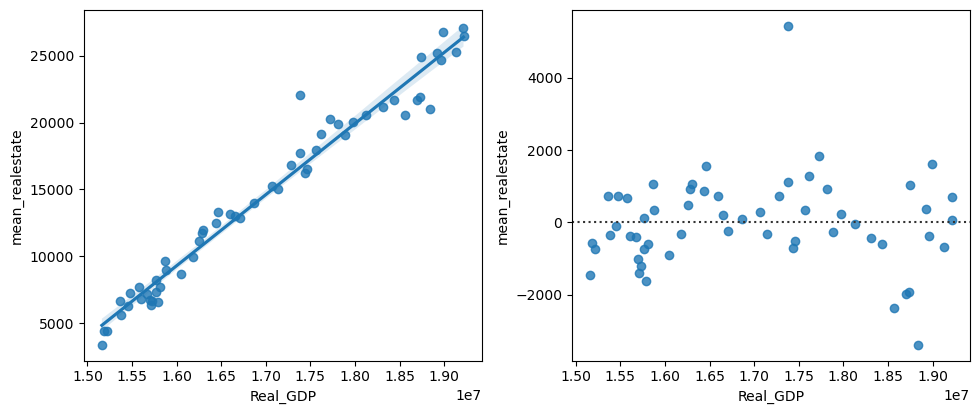
\includegraphics[width=1\textwidth]{imagens/Real_Estate.png}
    \caption{Regression and residual plot for the Real Estate sector}
    \label{something}
  \end{figure}

\begin{itemize}
    \item Positive significant effect
    \item Possible homoscedasticity
\end{itemize}
\end{frame}


\section{Conclusion}

\begin{frame}{Conclusion}

 \begin{itemize}
        \item Real GDP statistically significant positive effect on average market capitalization in sectors Communication Services and Real Estate
        \begin{itemize}
        \item Communication Services no sign of homoscedastictiy
        \item Real Estate shows possible homoscedasticity
        \end{itemize}
\end{itemize}
 \begin{itemize}
 \item Control variables:
        \begin{itemize}
        \item Unemployment Rate statistically significant effect in sectors Consumer Staples, Energy, Industrials and Real Estate
        \item Crude Prices statistically significant effect in sectors Communication, Energy, Health Care, Industrials and Materials
        \item Federal Debt statistically significant effect in all sectors except Energy and Financials 
        \item Federal Rate statistically significant effect in all sectors except Energy 
        \end{itemize}
\end{itemize}

\end{frame}

\section{References}
\begin{frame}{References}
Data sources:
\begin{itemize}
    \item https://fred.stlouisfed.org/
    \item  Bloomberg
\end{itemize}
\end{frame}

\begin{frame}{}

\begin{center}

    Thank you for your attention!
\end{center}

\end{frame}

\end{document}